\chapter{Simulation Study} \label{chapter3:Simulation-Study}

In this chapter we will present some results that support the claim that the various estimators discussed in Chapter~\ref{chapter2:Procedure} are consistent.

First, assume we observe $\bm{y} = (y_1, \dots, y_{400})^T$ from a Gaussian process where the covariance function is Mat\'{e}rn (see \eqref{eq:matern}) with known parameters $\nu$, $\rho$, and $\sigma$. The observations come from locations $\bm{s}_1, \dots, \bm{s}_{400}$ spread randomly over the unit square in $\mathbb{R}^2$. Because we know $C(h)$, we can calculate the covariance matrix exactly:
\[
	\bm{\Sigma}_{ij} = C(||\bm{s}_i - \bm{s}_j||).
\]
From this we can find the exact likelihood.

It can be shown that for a Mat\'{e}rn covariance function like \eqref{eq:matern}, we can write the spectral density in closed form.
\[
	f(\omega) = \frac{\sigma g(\nu, \rho)}{\left( \frac{4\nu}{\rho^2} + \omega^2 \right)^{\nu+d/2}},
\]
where $d = 2$ is the dimension of the spatial domain and
\[
	g(\nu, \rho) = \frac{\Gamma\left(\nu + \frac{d}{2}\right)(4\nu)^\nu}{\pi^{d/2} \rho^{2\nu} \Gamma(\nu)}.
\]
Because we can calculate the spectral density directly in this scenario, we can avoid fitting the splines and estimating $\bm{\beta}$. By bypassing this step, we test just the procedures for sampling from $f(\omega)$ and estimating the $\Sigma_{ij}$.

To perform the test, we chose two values for $\nu$ and six values for $\rho$. The $\sigma$ parameter just controls the variance $\textrm{Var}(\bm{Y}(\bm{s}))$, and so it does not factor into the estimation of $\Sigma_{ij}$ for $i \neq j$. For each combination of parameter settings, we generated 100 Gaussian process realizations and compared the true and estimated log likelihoods. The results are summarized in Figure~\ref{fig:liks_by_rho}. Note that the estimated likelihoods are close to their true values in all cases, and the choice of $\rho$ does not appear to significantly affect the accuracy.

\begin{figure}[!htb]
	\centering
	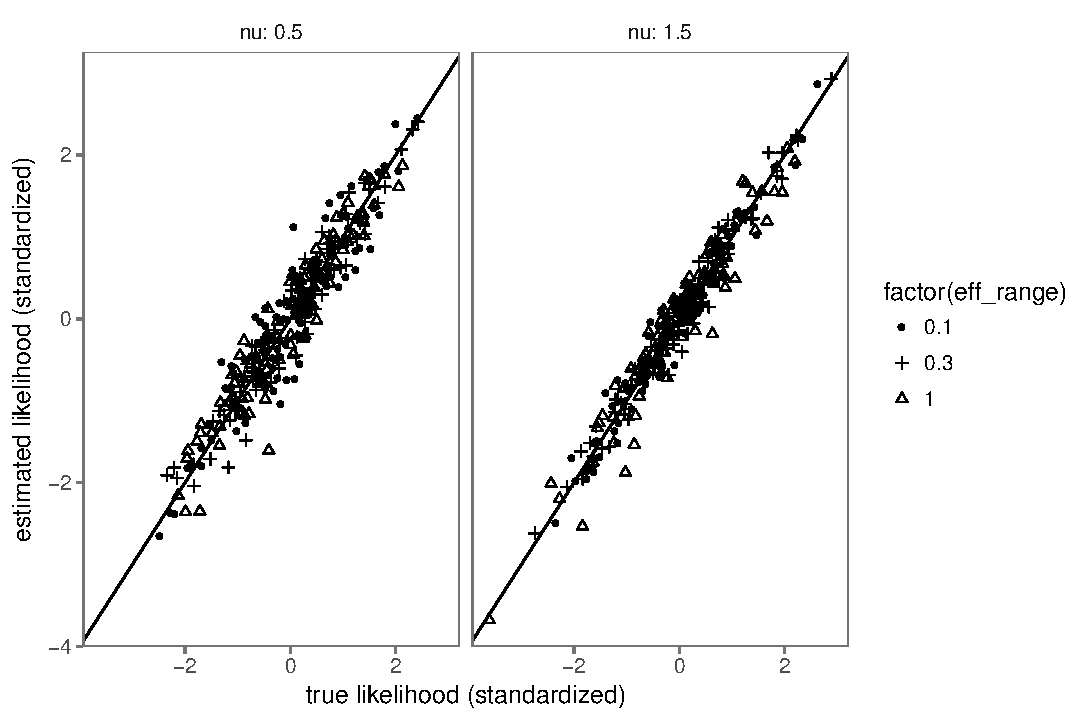
\includegraphics[width=0.95\textwidth]{lik_true_vs_est.pdf}
	\caption{\small Comparing true and estimated log likelihoods for varying values of $\rho$ (given above each plot). Values in each plot were centered and scaled for easier comparison. The likelihoods for the two values of $\nu$, $0.5$ and $1.5$, yield a similar pattern.}
	\label{fig:liks_by_rho}
\end{figure}

We ran a second version of this test that incorporated the $\bm{\beta}$ estimation. Still assuming the true $f(\omega)$ is known, we took 50 equally spaced points along $\log f(\log \omega)$ and fit natural splines to those points. This gave me some $\bm{\beta}_{\textrm{opt}}$, the values for $\bm{\beta}$ that most closely approximate $\log f(\log \omega)$. Then using $\bm{\beta}_{\textrm{opt}}$ we estimated the likelihood and again compared it to the true likelihood. Results are shown in Figure~\ref{fig:estliks_spline_rho}. The estimated likelihoods are still comparable to their true values, despite the fact that we are sampling from an approximation to $f(\omega)$ rather than $f(\omega)$ itself.

\begin{figure}[!htb]
	\centering
	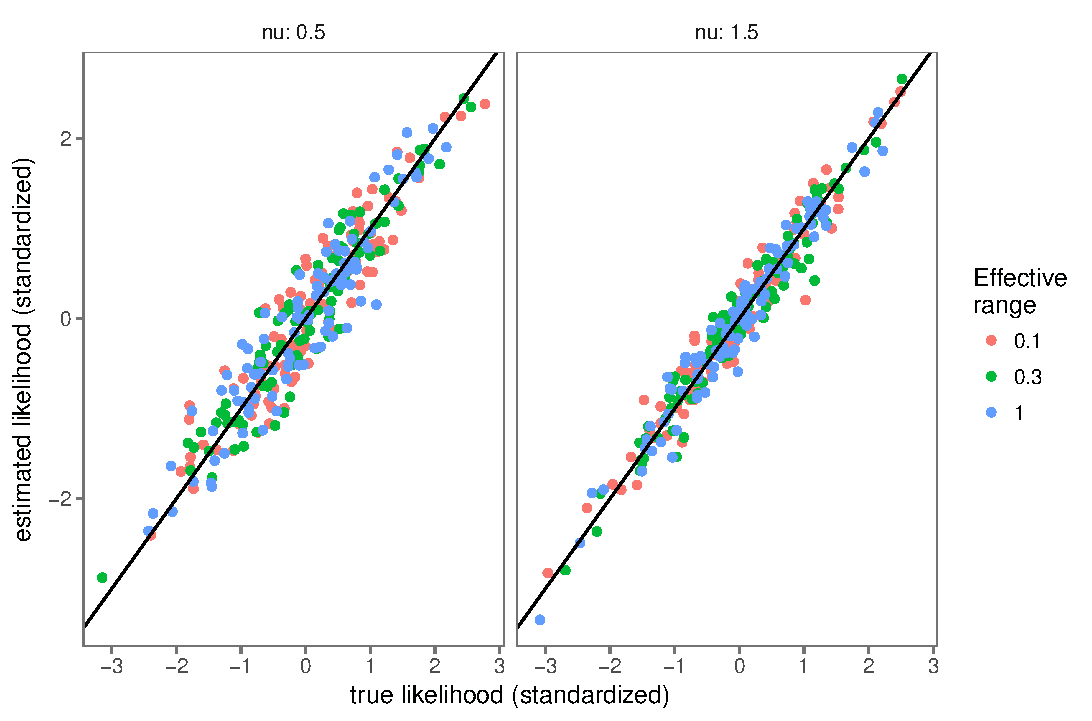
\includegraphics[width=0.95\textwidth]{lik_true_vs_est2.pdf}
	\caption{\small Comparing true and estimated log likelihoods for varying values of $\rho$ (given above each plot). Unlike the results in Figure~\ref{fig:liks_by_rho}, these estimates were generated not by sampling from $f(\omega)$ directly, but by sampling from a density approximating $f(\omega)$ fit using splines.}
	\label{fig:estliks_spline_rho}
\end{figure}

Finally, we put the entire procedure from Algorithm~\ref{alg:mcmc} into motion. First, $n = 400$ observations $\bm{y} = (y_1, \dots, y_{400})^T$ are drawn from a Gaussian process with a Mat\'{e}rn covariance function with $\nu = 1.5$, $\rho = 0.1548$, and $\sigma = 1$. This particular value of $\rho$ was chosen to obtain an effective range of 0.3. The observation locations are randomly spread across the unit square in $\mathbb{R}^2$ (see Figure~\ref{fig:locations}). An arbitrary initial $\bm{\beta}_0$ is chosen, and Algorithm~\ref{alg:mcmc} is run for $10000$ iterations. At each iteration, one likelihood calculation is made, using $M = 50000$ samples from the estimated spectral density $\hat{f}(\omega)$. After the chain is finished, the accepted $\bm{\beta}$ values are samples from the posterior distribution of $\bm{\beta} \;|\; \bm{y}$. After throwing away the first $2000$ values in the chain as burnin, the posterior mean $\widehat{\bm{\beta}}$ is chosen to be the best estimate of the true $\bm{\beta}$.

We chose a normal random walk proposal distribution for both the $\bm{\beta}$ and $\tau^2$ updates. Because it is symmetric, we were able to omit it from the calculation of $a$ in Algorithm~\ref{alg:mcmc}. We also used adaptive tuning to adjust the hyperparameters so that the acceptance rates stayed within an acceptable range.

Because we know the true $f(\omega)$, we can compare the spectral density approximated with $\widehat{\bm{\beta}}$ with the actual one. See Figure~\ref{fig:result} for that comparison. Figure~\ref{fig:result-covar} shows that the estimated covariance function agrees with the actual covariance function.


\begin{figure}[!htb]
	\centering
	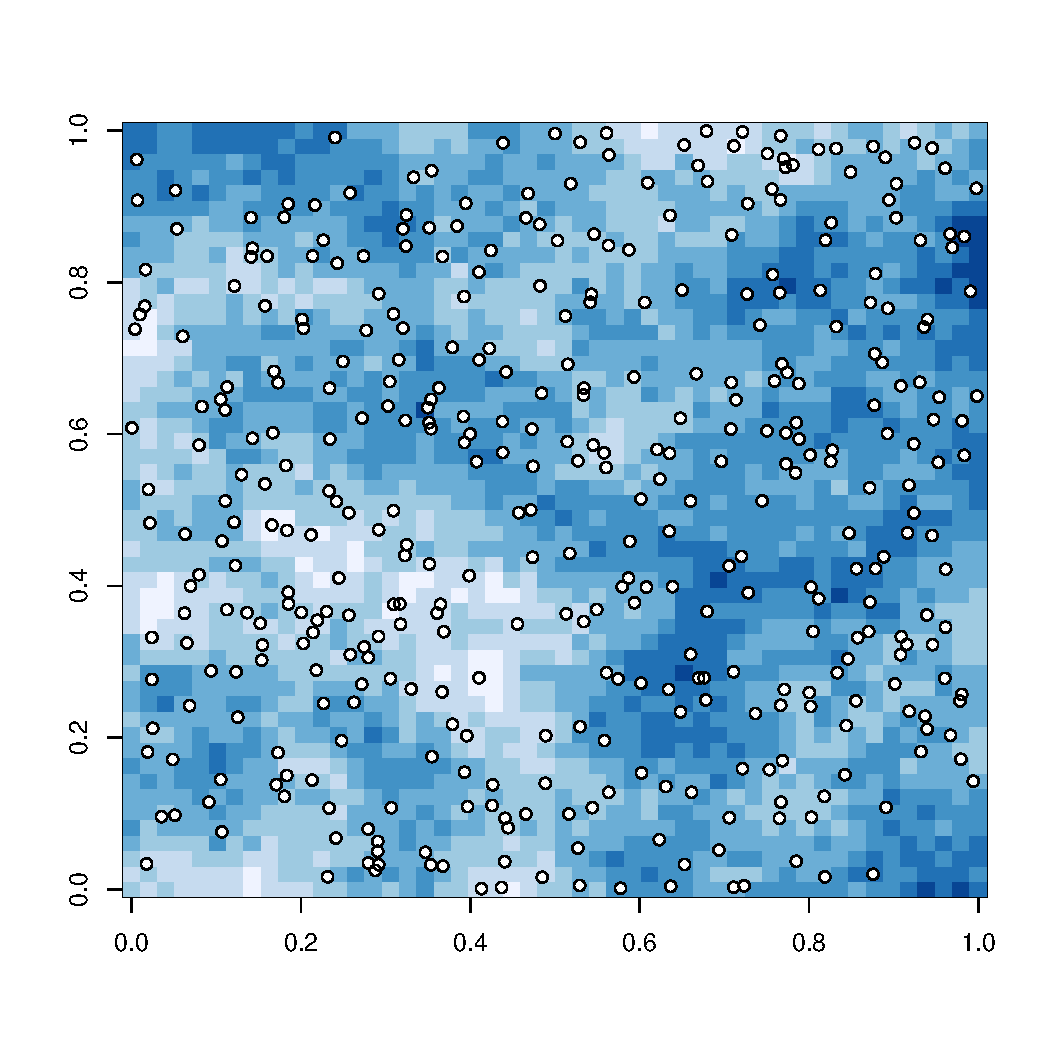
\includegraphics[width=0.95\textwidth]{locations.pdf}
	\caption{\small The locations $\bm{s}_1, \dots, \bm{s}_{400} \in \mathbb{R}^2$ of the observations from a Gaussian process with $\nu = 1.5$, $\rho = 0.1548$, and $\sigma = 1$. The locations are random, but generated in such a way that ensures the minimum distance between any two points is greater than $0.005$.}
	\label{fig:locations}
\end{figure}

\begin{figure}[!htb]
	\centering
	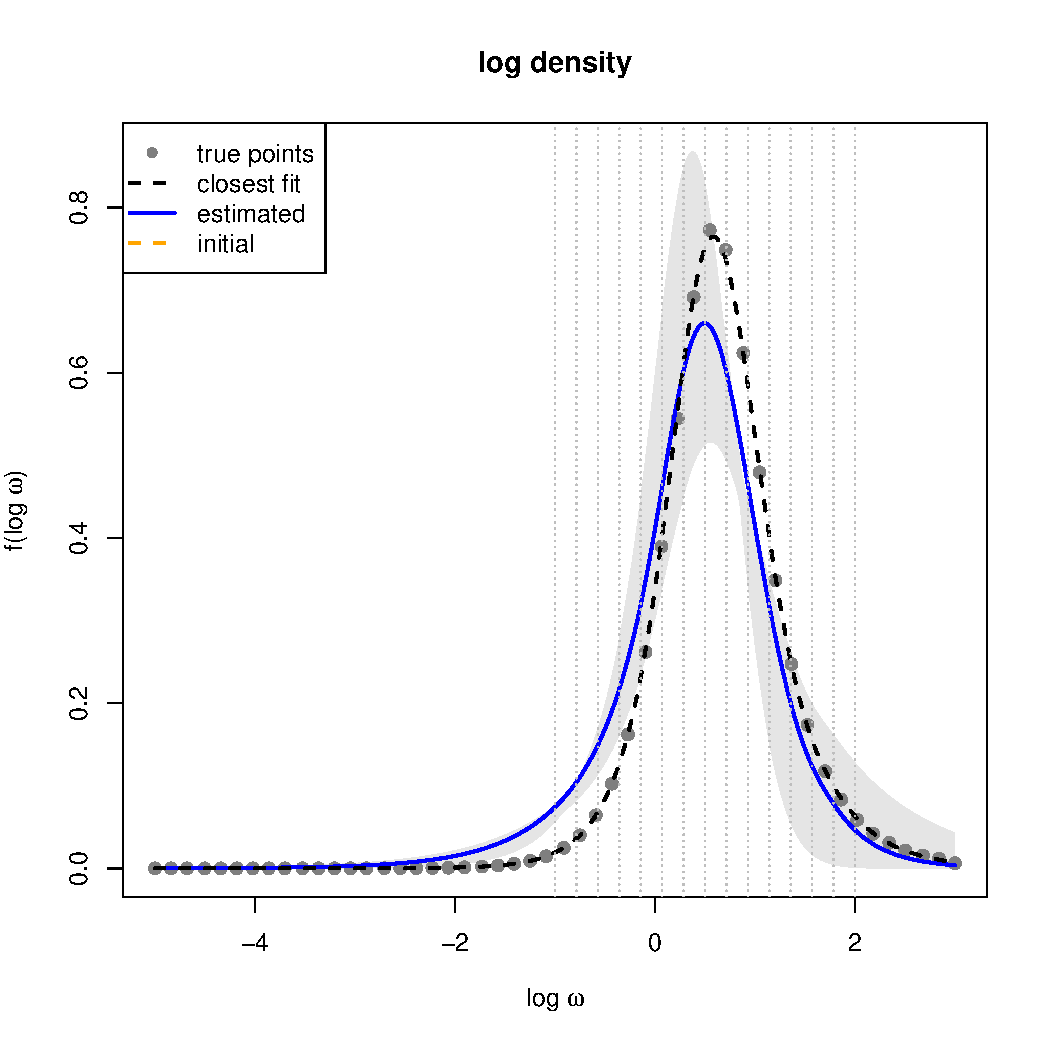
\includegraphics[width=0.95\textwidth]{logdensity.pdf}
	\caption{\small The actual $f(\log \omega)$ (black) versus the estimated $\hat{f}(\omega)$ (blue). The yellow dotted line is the curve from the initial values of the spline coefficient; it is included to illustrate the MCMC algorithm converging to the correct result. The shaded area represents the range of the middle 95\% of $\hat{f}(\omega)$ for all draws from $\bm{\beta} \;|\; \bm{y}$. The vertical gray dotted lines indicate where the knots were placed.}
	\label{fig:result}
\end{figure}

\begin{figure}[!htb]
	\centering
	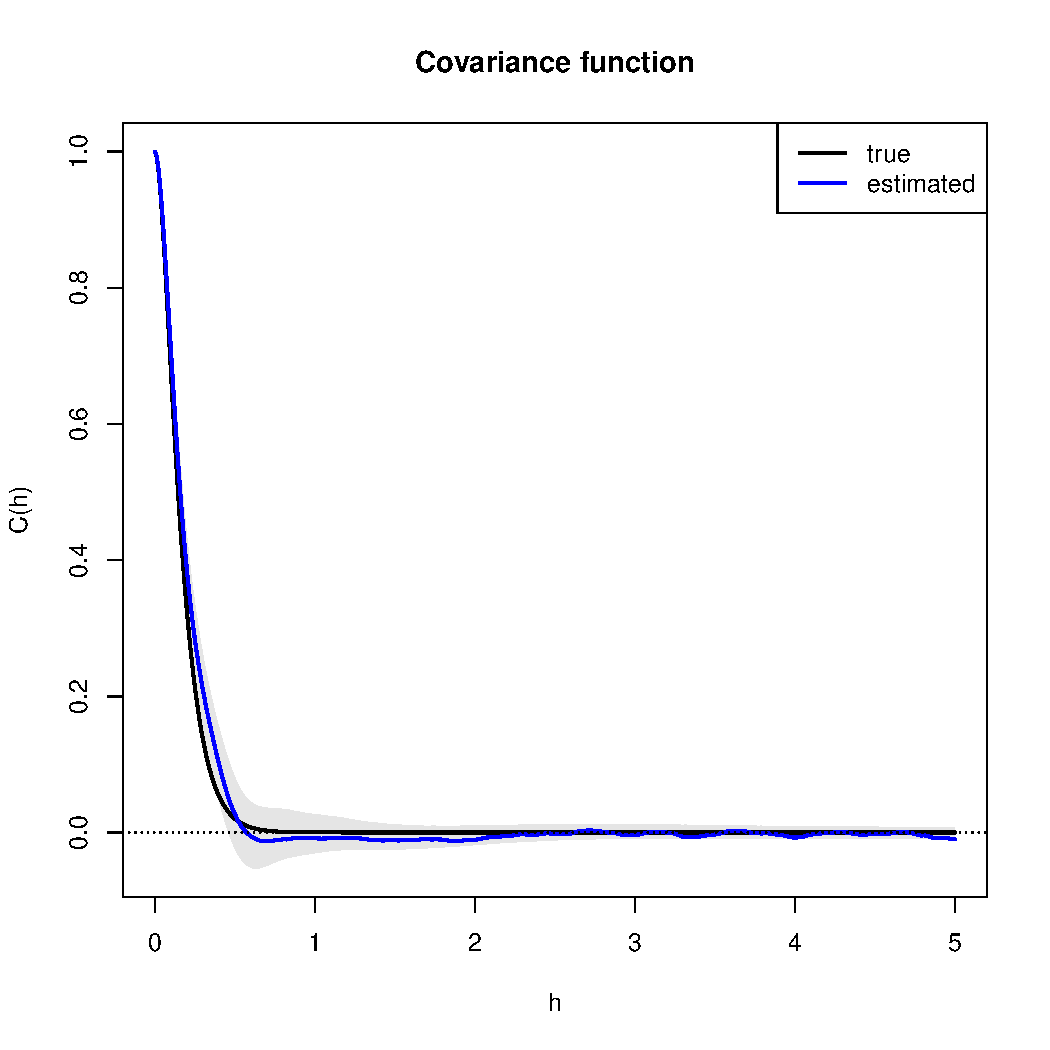
\includegraphics[width=0.95\textwidth]{covar.pdf}
	\caption{\small The actual $C(h)$ (black) versus the estimated $\widehat{C}(h)$ (blue). The shaded area represents the range of the middle 95\% of $\widehat{C}(h)$ for all draws from $\bm{\beta} \;|\; \bm{y}$.}
	\label{fig:result-covar}
\end{figure}

% subsection consistency_of_the_likelihood_estimate (end)